\documentclass[../design.tex]{subfiles}

\begin{document}
\section{Frontend structure}
The frontend structure has already been introduced in previous sections,
however, the goal of this section is to provide a deep dive into the decisions
that have led to the chosen structure. Furthermore, as this thesis is based in
the frontend application development, it is more explanatory than the backend
structure section.
\subsection{Initial challenges}
Before defining how would the repository or repositories of the frontend would
be, a first challenge arose regarding the usage of hexagonal architecture.
\\
While the hexagonal architecture can be applied to various types of
applications, including frontend applications, it is not commonly used in modern
frameworks like React and Vue\footnote{React and Vue have been used as the
	example as they are the two of the most popular frontend frameworks nowadays. It
	is important to note that most of the challenges explained in this section could
	apply to any component-based frontend framework.}. There are a few reasons for
this:
\begin{enumerate}[label = -]
	\item\textbf{Simplicity and ease of use}: Frameworks like React and Vue are
	designed to provide a simplified and intuitive approach to building user
	interfaces. They prioritize ease of use and developer productivity by
	providing a clear and straightforward programming model. The hexagonal
	architecture, on the other hand, introduces additional complexity and
	layers of abstraction, which may not be necessary for the majority of
	frontend applications.
	\item\textbf{Focused on UI concerns}: Modern component-based frameworks are
	primarily focused on managing the user interface and handling the view
	layer of an application. They provide features and abstractions that are
	specifically tailored for building interactive and dynamic user
	interfaces. The hexagonal architecture, on the other hand, is more
	concerned with the separation of concerns and the decoupling of business
	logic from infrastructure, which may not be the primary focus of frontend
	frameworks.
	\item\textbf{Component-based architecture}: React and Vue are based on a
	component-based architecture, where the user interface is broken down into
	reusable and composable components. This approach aligns well with the
	principles of modularity and reusability but does not necessarily require
	the level of decoupling provided by the hexagonal architecture. The focus
	in frontend frameworks is often on managing the relationships and
	interactions between components rather than on separating business logic
	from infrastructure.
	\item\textbf{Limited backend integration}: Frontend frameworks typically
	interact with backend APIs or services to fetch data and perform actions.
	The hexagonal architecture is more commonly applied in scenarios where
	there is a need to integrate with various external systems and
	dependencies, such as databases, third-party APIs, or messaging systems.
	In frontend applications, the emphasis is usually on consuming APIs
	provided by the backend rather than managing complex integration
	scenarios.
\end{enumerate}
While the hexagonal architecture may not be commonly used in component-based
frontend frameworks, like React and Vue, it can still be beneficial in certain
cases, especially when building large and complex frontend applications that
require a high level of modularity, testability, and extensibility. However,
it's important to consider the trade-offs in terms of complexity and developer
experience before adopting this architecture in a frontend context.
\\[8pt]
Taking this into account, two options software design ideas were over the table:
\begin{enumerate}
	\item Finding a code structure that would allow the developers to apply most
	      of the hexagonal architecture patterns.
	\item Not applying hexagonal architecture patterns and sticking to
	      having business logic within the frontend.
\end{enumerate}
Obviously each option has advantages and disadvantages. Therefore, in order to
decide which option was more suitable or preferred for the current case, I
answered the following questions, for each possibility:
\begin{enumerate}
	\item How easy to extend the domain for the option is?
	      \begin{enumerate}[label = -]
		      \item\textbf{HA\footnote{Stands for \emph{Hexagonal
					      Architecture}}}: Straightforward, as it is one of the main ideas
		      of such architecture.
		      \item\textbf{NHA\footnote{Stands for \emph{Non-Hexagonal
					      Architecture}}}: Can be on both edges. If domain is
		      fairly small and modular, it can easily be extended. On the other
		      hand, it can be a nightmare for developers incrementing the time
		      for changes and increasing the possibility of side effects.
	      \end{enumerate}
	\item How easy would it be to share the domain with another frontend
	      application?
	      \begin{enumerate}[label=-]
		      \item \textbf{HA}: Straightforward, as the domain is decoupled from the
		            framework and can be shared with other frontend applications
		            easily, without the need of any modification. The domain of
		            the frontend must be frontend framework-agnostic.
		      \item \textbf{NHA}: Difficult, as the business logic is tightly coupled
		            with the frontend framework, making it challenging to extract and
		            share the domain with other applications. Moreover, each
		            framework may have different methods to separate business
		            logic from components, making these methods non-compatible
		            between each framework.
	      \end{enumerate}
	\item How attached is the domain to the framework?
	      \begin{enumerate}[label=-]
		      \item \textbf{HA}: Loosely coupled, as the domain is decoupled from the
		            framework, allowing for easy substitution or changes to the
		            frontend framework.
		      \item \textbf{NHA}: Tightly coupled, as the business logic is entangled
		            with the frontend framework, making it difficult to switch or adapt
		            to a different framework.
	      \end{enumerate}
	\item What is the quality of the \emph{frontend} developer experience?
	      \begin{enumerate}[label=-]
		      \item \textbf{HA}: Generally positive, as the hexagonal architecture
		            promotes clean separation and modularity, which can enhance the
		            developer experience in understanding and maintaining the codebase.
		      \item \textbf{NHA}: Variable, as the lack of clear separation between
		            business logic and frontend concerns can lead to a steeper learning
		            curve and potential challenges in maintaining and evolving the
		            application.
	      \end{enumerate}
	\item How likely is it to increase the frontend bundle size, therefore,
	      \emph{decreasing user experience}?
	      \begin{enumerate}[label=-]
		      \item \textbf{HA}: Less likely, as the hexagonal architecture promotes
		            modularity and the separation of concerns, which can lead to more
		            efficient code and better control over the bundle size.
		            Nonetheless, it requires a strict analysis to the code and
		            bundle size, in order to split as much code as possible,
		            ensuring the minimal bundle size. Furthermore, utilities
		            such as lazy loading and server-side rendering can also have
		            a huge impact on user experience.
		      \item \textbf{NHA}: More likely, as the business logic being tightly
		            coupled with the frontend framework may result in larger bundle
		            sizes, potentially affecting the user experience. However,
		            lazy loading and server-side rendering can reduce the amount
		            of JS sent to the client, thus reducing the latency for the
		            page to load. Furthermore, configuration would be less
		            complex as in the \textbf{HA} approach, were multiple
		            bundles would have to be configured, as well as proper
		            configuration to serve such bundles.
	      \end{enumerate}
	\item In case of incorporating new teammates into the codebase, how likely
	      is it for new developers to understand and quickly start working with it?
	      \begin{enumerate}[label=-]
		      \item \textbf{HA}: More likely, as the hexagonal architecture provides a
		            clear separation of concerns, making it easier for new developers to
		            understand and contribute to the codebase.
		      \item \textbf{NHA}: Less likely, as the lack of separation between
		            business logic and frontend concerns may require new developers to
		            spend more time grasping the codebase and its intricacies.
	      \end{enumerate}
	\item In the case of an application that requires to be developed as soon as
	      possible, how time-consuming is this methodology?
	      \begin{enumerate}[label=-]
		      \item \textbf{HA}: The hexagonal architecture, with its focus on
		            separation of concerns and modular design, may require
		            additional upfront planning and design efforts. Even more in an
		            environment that is not thought to support or simplify the
		            application of such patterns or methodologies. Implementing the
		            necessary layers and abstractions can take more time compared to
		            a more straightforward approach. However, it can provide
		            benefits in the \emph{long term}, such as easier maintenance and
		            extensibility.
		      \item \textbf{NHA}: Not applying the hexagonal architecture patterns and
		            having business logic within the frontend can allow for faster
		            development initially, as there are fewer layers and abstractions to
		            set up. However, it may lead to challenges in the long run, such as
		            increased code complexity and difficulties in maintaining and
		            extending the application.
	      \end{enumerate}
\end{enumerate}
Taking into account the previous answers, the hexagonal architecture has been
chosen despite the potential challenges and complexities that may occur when
defining and designing the codebase architecture. The decision to prioritize HA
is based on the following reasons:
\begin{enumerate}
	\item\textbf{Extensibility}: The hexagonal architecture approach provides a
	structured and modular approach to software design, enabling easier
	extension of the domain and incorporation of new features or changes in
	the future. By separating the core business logic from external
	dependencies and infrastructure concerns, the application becomes more
	flexible and adaptable to evolving requirements.
	\item\textbf{Code reusability and sharing}: The hexagonal architecture
	allows the domain logic to be decoupled from the frontend framework,
	facilitating sharing of the domain with other frontend applications or
	even backend systems. This promotes code reuse, improved collaboration
	between teams, and faster development in the long run.
	\item\textbf{Maintainability and Testability}: The clear separation of
	concerns in hexagonal architecture enhances maintainability and
	testability. With a well-defined architecture, it becomes easier to write
	unit tests for the core business logic and make changes without affecting
	other parts of the application. This improves code quality, reduces bugs,
	and enhances overall software stability.
	\item\textbf{Developer Experience}: Although implementing the hexagonal
	architecture may require more initial effort, it promotes clean code
	organization, modularity, and a better understanding of system boundaries.
	This contributes to a more pleasant and productive developer experience,
	particularly for larger and more complex projects.
	\item\textbf{Future-proofing}: By adopting the hexagonal architecture, the
	application becomes less tightly coupled to the frontend framework, reducing
	the risk of vendor lock-in and providing more flexibility to adapt to future
	changes, such as switching to a different framework or adopting new
	technologies.
\end{enumerate}
The decision to choose hexagonal architecture acknowledges the challenges
involved but prioritizes long-term benefits such as extensibility, code
reusability, maintainability, and improved developer experience. It aims to
create a robust and adaptable software architecture that can evolve with the
changing needs of the application and provide a solid foundation for future
development.
\subsection{Architecture solution}
Being someone who has never had professional experience on working in projects
that use hexagonal architecture or a variant of it, it was quite a challenge to
define a software architecture that would work with the hexagonal architecture.
Some aspects about the architecture were clear:
\begin{enumerate}
	\item There should be a package or a module that will include the domain of
	      the enterprise. This domain \textbf{must} be independent of the UI logic,
	      therefore, frontend framework independent.
	\item The frontend implementation should use the infrastructure layer of the
	      domain module, which will abstract the business logic, therefore completely
	      removing domain business logic from the frontend.
\end{enumerate}
It is important to differentiate between the domain business logic, which should
not have any relation with the frontend framework, from the user interface (or
view) business logic, which may be state management and similar, necessary to
ensure the application works, while being independent of the domain.
\\[8pt]
In addition, it is essential to have a design system or component library that
is attached to the frontend framework but agnostic to the specific domain. This
entails the existence of at least one package per framework used in any frontend
application, providing a collection of base components (such as input fields,
dialogues, and buttons) that can be utilized across different apps. For instance,
if there is a React application, it should have a React component library that
is designed to be extendable and modular, allowing for reusability throughout
the entire enterprise. This component library serves as a centralized repository
for commonly used UI components, ensuring consistency in design and user
experience across different applications built with the same frontend framework.
\\
Even though these libraries will not follow a hexagonal architecture from top to
bottom, they will take advantage of some of its principles.
\\[8pt]
Finally, each frontend application will combine the shared domain, the shared
components, and its specific framework implementation.
\subsection{Domain architecture}
The domain has to be understood as a package, even though it uses the same
naming as the \emph{domain} from the hexagonal architecture principles. The
domain package it is separated in three layers: domain, application, and
infrastructure. Each layer corresponds to each layer in the hexagonal
architecture and is going to be developed accordingly. However, the
infrastructure layer is slightly different from it commonly is. Normally, the
last layer of the HA\footnote{Hexagonal architecture, for short} is the
infrastructure, yet in this specific design, it will only be the last layer of
the domain package. This last layer is going to be used in the frontend, which
is the last layer of the architecture, as the frontend will always be above the
architecture.
\begin{figure}[H]
	\centering
	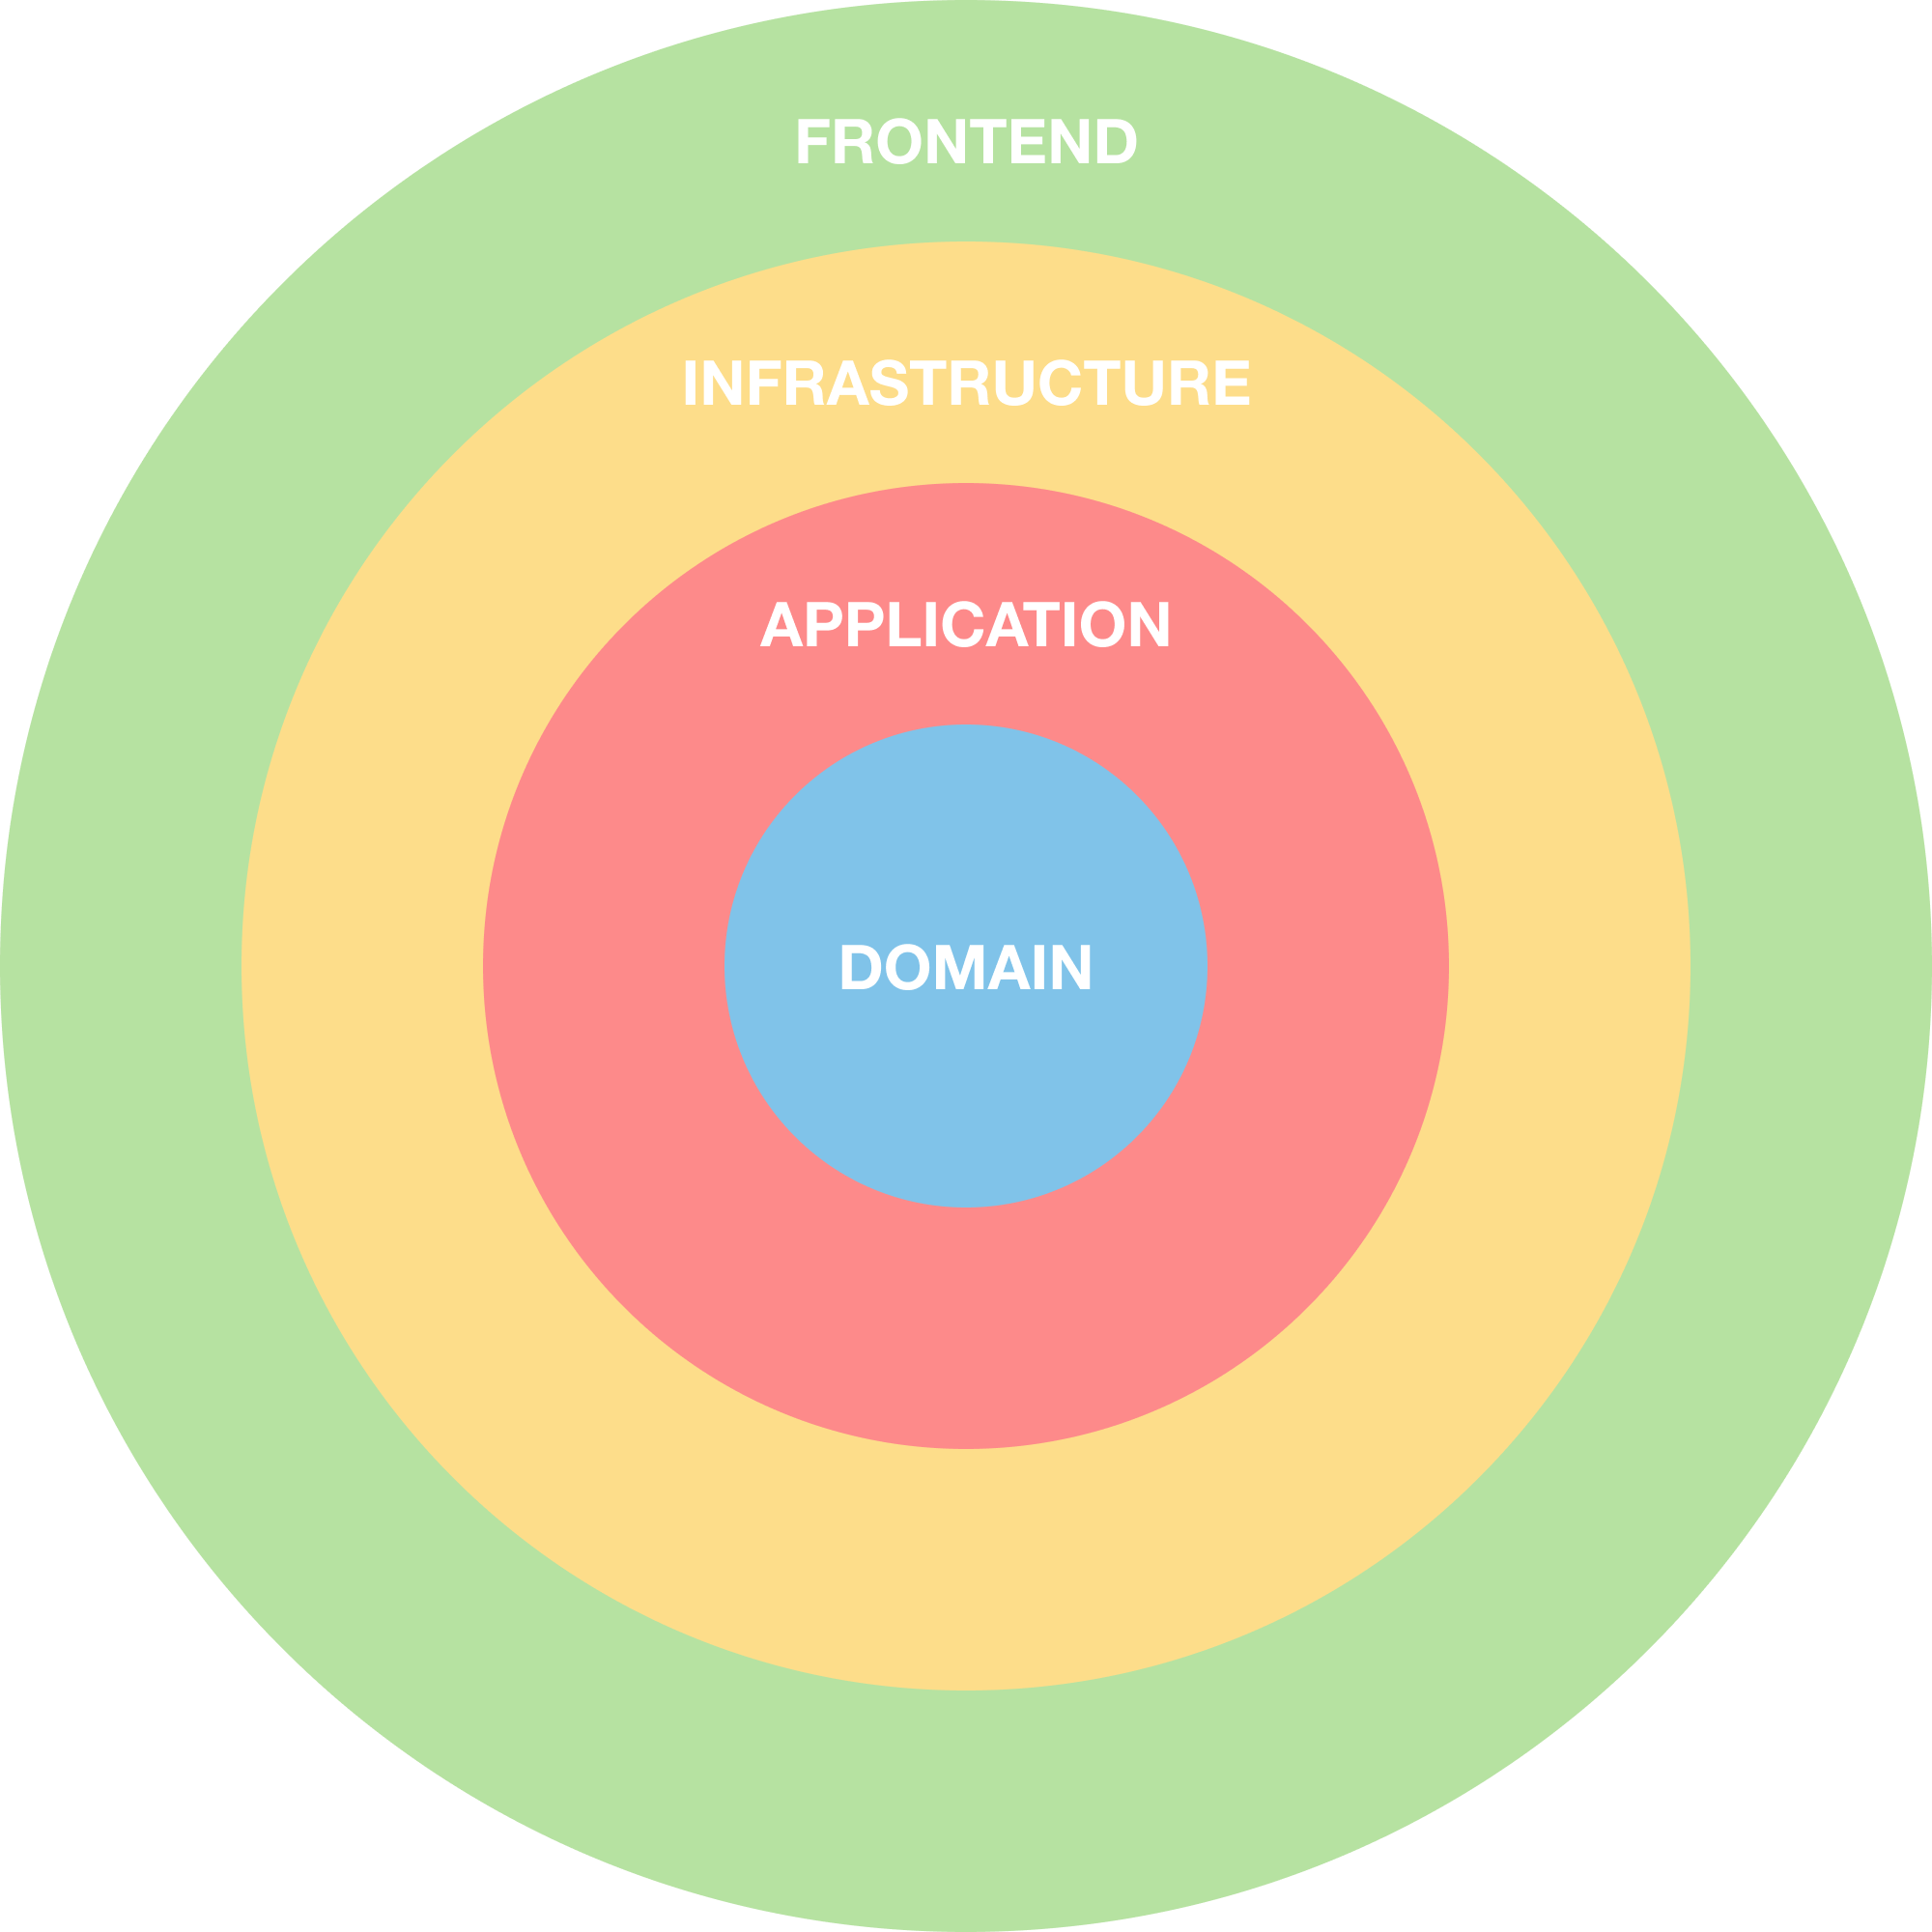
\includegraphics[width=0.5\textwidth]{./assets/ha.png}
	\caption{Four layer hexagonal architecture}
\end{figure}
As explained previously, the domain must be frontend framework independent,
therefore it should not know anything about what is in the outer layer. This
respects to the hexagonal architecture principles and allow us to have a domain
package that can be shared by many frontends, independent of their technology.
\subsubsection{Infrastructure layer}
The application layer has little to add, since it does not differ an
implementation that can be found in other projects that use hexagonal
architecture.
\\[8pt]
Delving deeper into the structure of the domain package, the domain and
application layers have been implemented following the principles of the
hexagonal architecture (HA) from top to bottom. However, the infrastructure
layer has been slightly modified to better cater to potential frontend
requirements. For example, using the controller pattern wouldn't be suitable as
the package is not intended to be a REST API. Instead, it should provide entry
points for the frontends to utilize the domain logic, such as data validation or
retrieval.
\\
The purpose of these entry points is to decouple the fetching function, which
can be implemented using either the native `fetch` function or a dedicated
package like \texttt{axios} from the frontend. The infrastructure layer of the
domain package will simply provide a function that utilizes an HTTP client to
communicate with an external server. The frontend can then make use of this
entry point without needing to be aware of the underlying implementation
details.
\\
This approach is crucial to minimize the domain-related business logic within
the frontend. It offers several benefits, including:
\begin{enumerate}
	\item\textbf{Reduced Dependencies}. By providing entry points that abstract away the
	specifics of data fetching and communication, the frontend application becomes
	less dependent on external libraries or frameworks. This results in a
	cleaner and more lightweight frontend codebase.
	\item\textbf{Simplified Testing}. With a decoupled infrastructure layer, testing
	becomes easier as the infrastructure can be easily mocked or replaced with
	test-specific implementations. This allows for more focused and efficient
	testing of the frontend logic without the need for complex setups or
	external dependencies.
	\item\textbf{Abstraction and Modularity}. The use of entry points abstracts away the
	implementation details of data retrieval, enabling the frontend to focus
	on using the domain logic without being concerned about the specific
	technologies or protocols involved. This abstraction enhances modularity
	and allows for easier future changes or updates to the infrastructure
	layer.
\end{enumerate}
By decoupling the frontend from domain-specific infrastructure concerns, the
application benefits from reduced dependencies, simplified testing, and improved
modularity. It ensures that the frontend remains focused on its primary
responsibilities while leveraging the domain logic through well-defined entry
points.
\\[8pt]
These entrypoints are exposed, as a package, named as queries. A query is a
function, as explained above, that can either be a validator (i.e. a validator
for an input field) or an HTTP client call (i.e. a function that fetches all the
travels from a user).
\\
To implement the contract of the domain, which is defined as an interface, the
queries need to adhere to this contract. Although queries are pure functions,
the interface must be implemented as a class. These classes, commonly referred
to as \emph{queriers} serve as the implementation of the domain contract.
\\
The queriers encapsulate the logic and operations specified by the domain
contract. They act as a bridge between the application layer and the queries,
ensuring that the queries align with the defined domain contract. By
implementing the domain contract within queriers, consistency and clarity in
code implementation are promoted.
\\
Queriers are designed as singletons, meaning that only a single instance of each
querier class is created and shared across the application. This singleton
approach provides memory efficiency, as there is no need to create multiple
instances of the same querier. It also simplifies the usage of queriers, as the
same instance can be reused in different use cases, promoting code reuse and
reducing duplication. Using queriers brings several benefits to the application:
\begin{enumerate}
	\item\textbf{Consistency}. By implementing the domain contract within
	queriers, all queries adhere to the same interface. This promotes
	consistency in how queries are structured and ensures that they fulfill the
	expected behaviour specified by the domain contract. This is one of the core
	principles of HA.
	\item\textbf{Code reusability}. Queriers can be reused across different use
	cases, allowing for efficient and modular development. The same querier
	instance can be utilized in multiple contexts, reducing code duplication
	and enhancing maintainability.
	\item\textbf{Memory efficiency}. Queriers as singletons optimize memory
	usage. With only one instance of each querier, unnecessary memory
	allocation is avoided, leading to better performance and resource
	management.
\end{enumerate}
Since DDD (domain-driven design) is used, this implementation allows the
developers to separate \emph{queries} and \emph{queriers} by domain, or even
bounded contexts\footnote{Since the application does not require the usage of
	bounded contexts, the packages have been separated by domain (i.e.
	authentication or travels) in a single bounded context}. The implementation of
multiple domains looks as:
\begin{figure}[H]
	\centering
	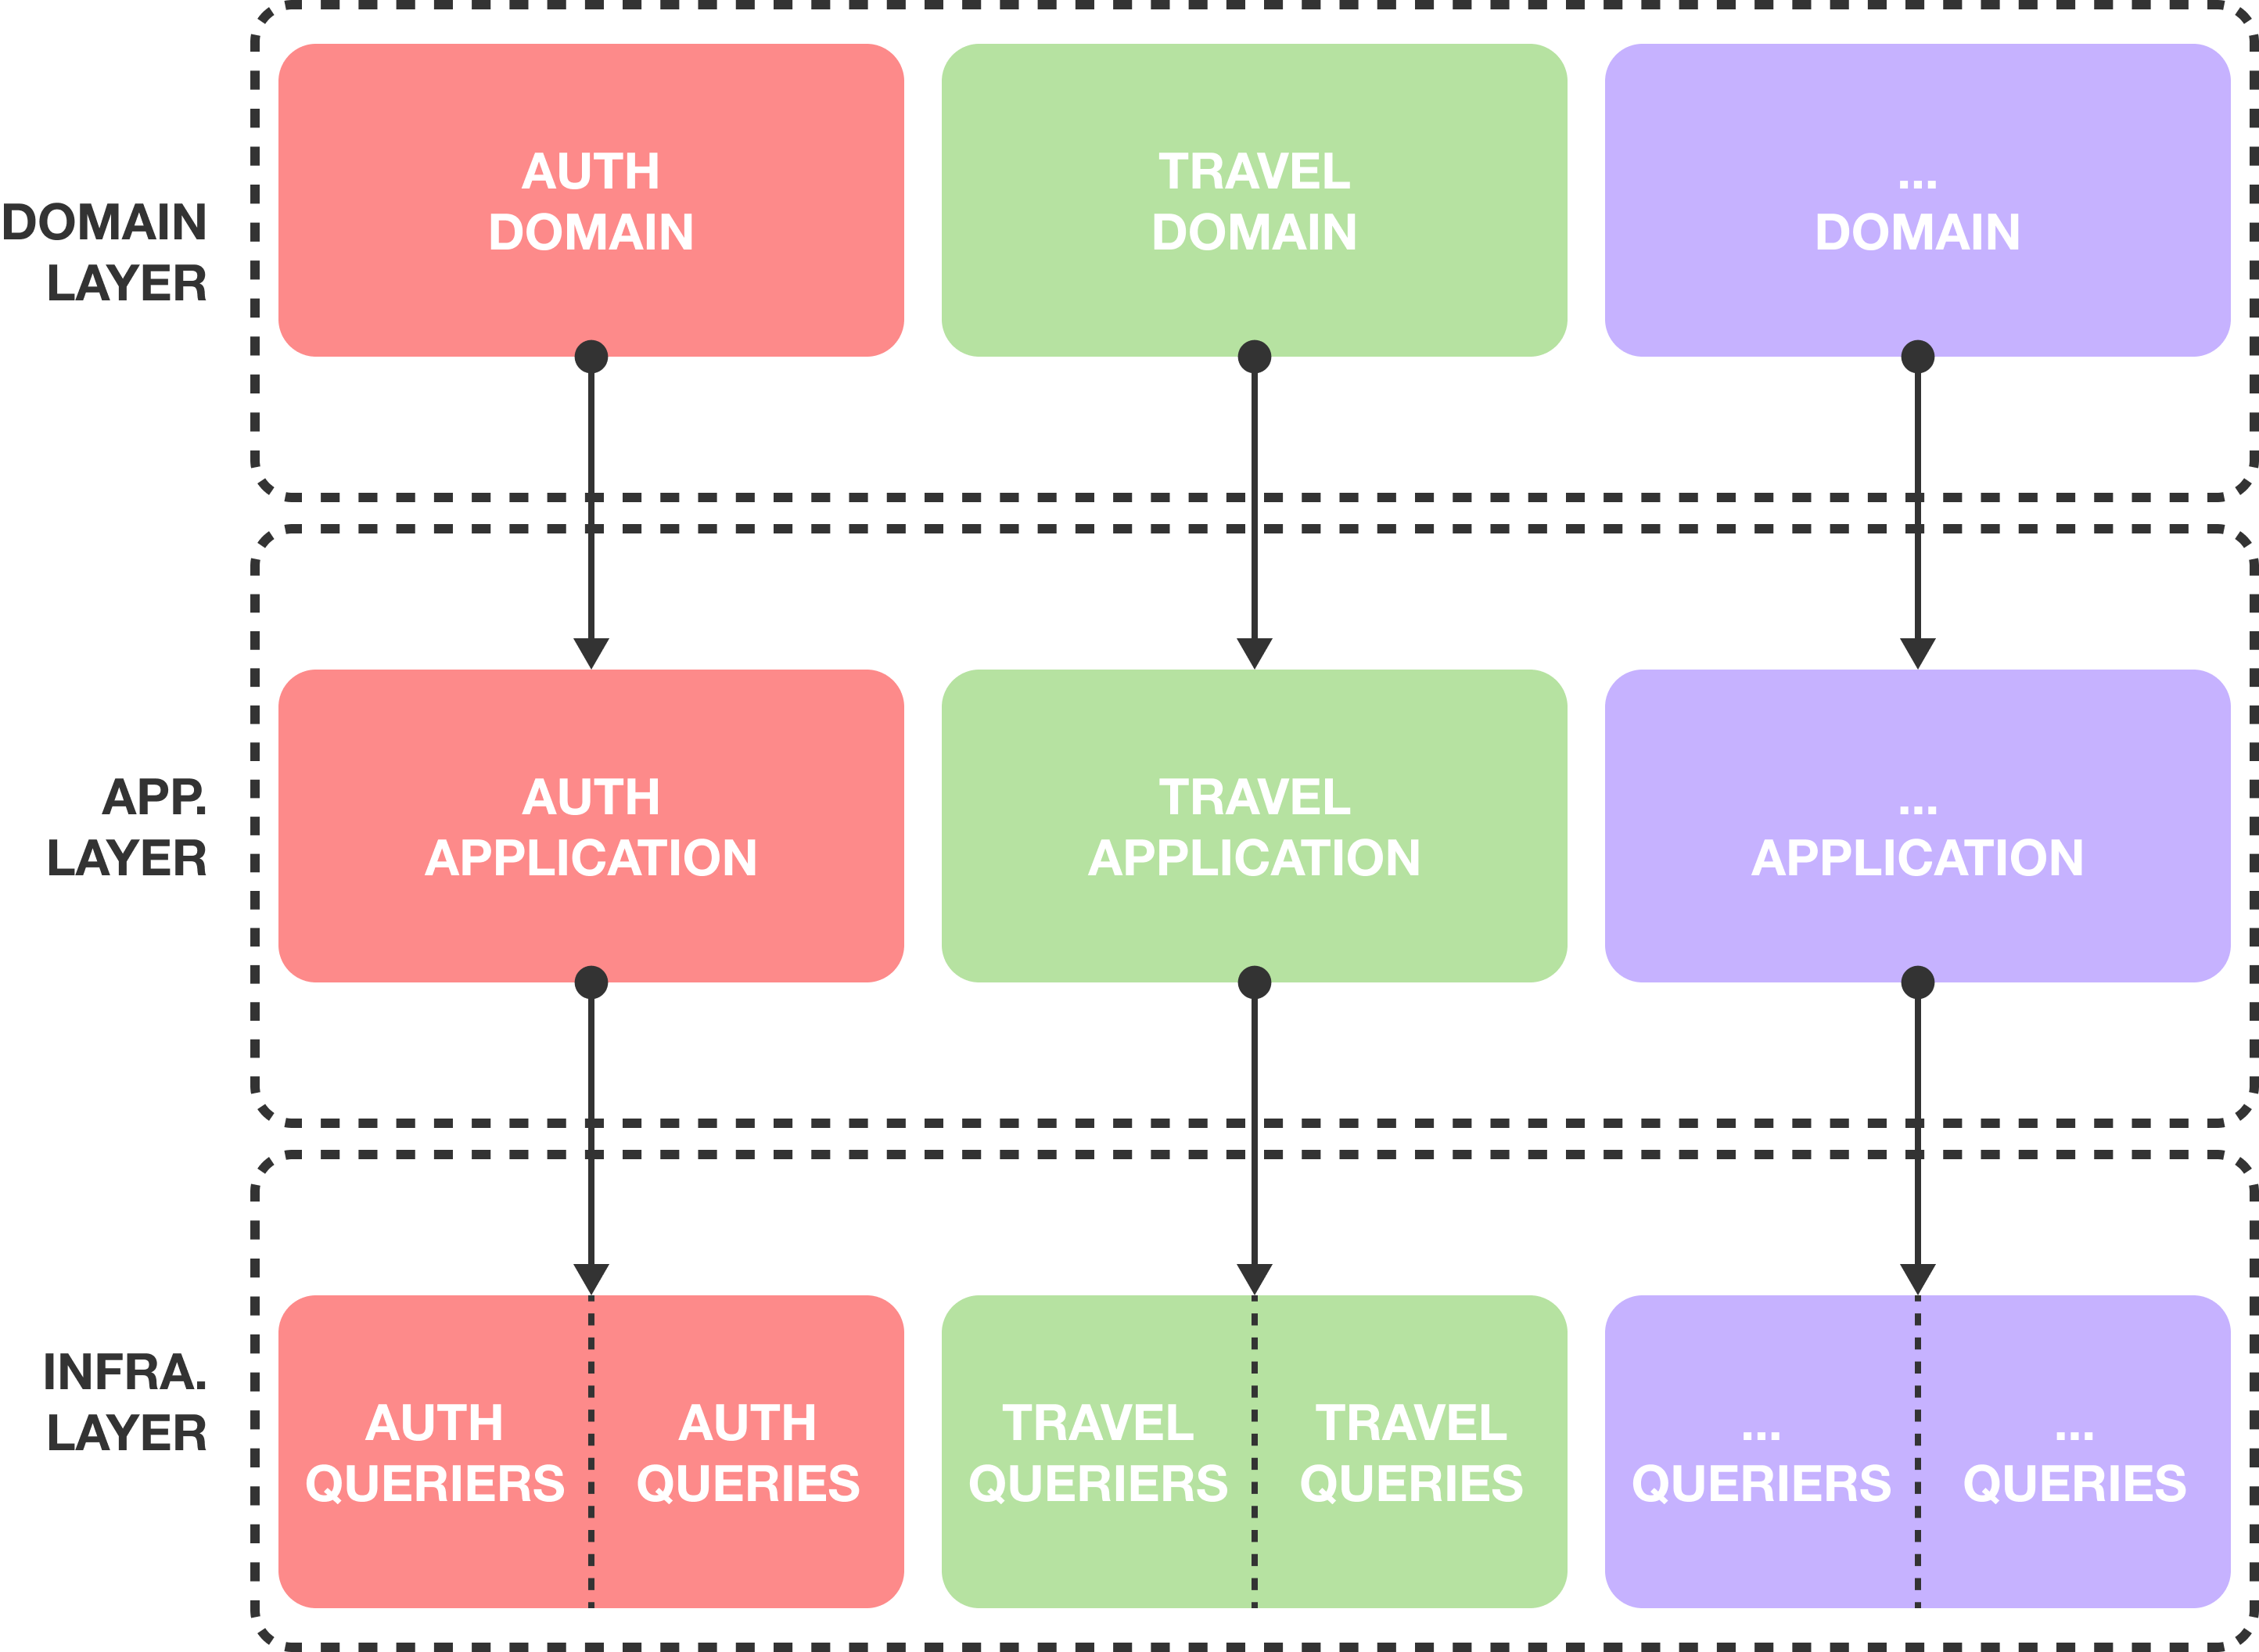
\includegraphics[width=0.75\textwidth]{./assets/core-multi-domain.png}
	\caption{Exemplification of the implementation of multiple domains in the
		proposed architecture.}
\end{figure}
It is important to mention that, ideally, domains \emph{should not interact
	between each other}.
\subsection{Shared components}
Once the domain architecture has been defined, the next step was to create an
internal package, within the monorepository, that would contain all the
components. Since the goal of this project is to also develop a scalable and
extendable architecture, it was decided to create a new UI module that would
have the implementation of the components from the "design system" for each
framework. For example, in this case, the UI package only contains a
sub-package, named \emph{react}, that will contain the implementation of the
components in order to be used in react applications.
\\
Moreover, this UI package can easily add another framework-dependent library, as
each library will be compiled and used independently. In the long term, the team
could have a unique design system, implemented in different languages or
frameworks.
\\[8pt]
These components should be domain independent, therefore they should as much
extendable as possible. With the appearance of React, component-based frameworks
have adopted the principle of \emph{composition over inheritance}. This
principle encourages building components by composing smaller, reusable
components instead of relying on inheritance. By following this principle,
components become more flexible, maintainable, providing easier extension and
customization.
\\
Looking for domain-independent components, composition over inheritance is
especially beneficial, as it enables the creation of components that can be
easily extended and combined to build complex user interfaces. Rather than
relying on a deep hierarchy of inheritance, components can be composed together,
utilizing their individual functionalities to create new, specialized
components.
\\
Furthermore, by utilizing composition, developers can leverage the power of
higher-order components\footnote{It is also important to mention that with the
	usage of React hooks, most frameworks are switching to a hook-based development,
	that reduces the usage of HOCs} (HOCs), render props, or hooks to enhance and
extend the behaviour of existing components. This approach allows for the
selective reuse of specific features or functionality, which also implies code
duplication reduction and increased code maintainability.
\\
Overall, by embracing the principle of composition over inheritance,
domain-independent components become more versatile, extensible, and modular.
This approach aligns with the component nature of frameworks like React
and Vue, enabling developers to build flexible and reusable UI components that
can adapt to various application requirements.
\\[8pt]
Taking into account our current architecture, by adding the component library:
\begin{figure}[H]
	\centering
	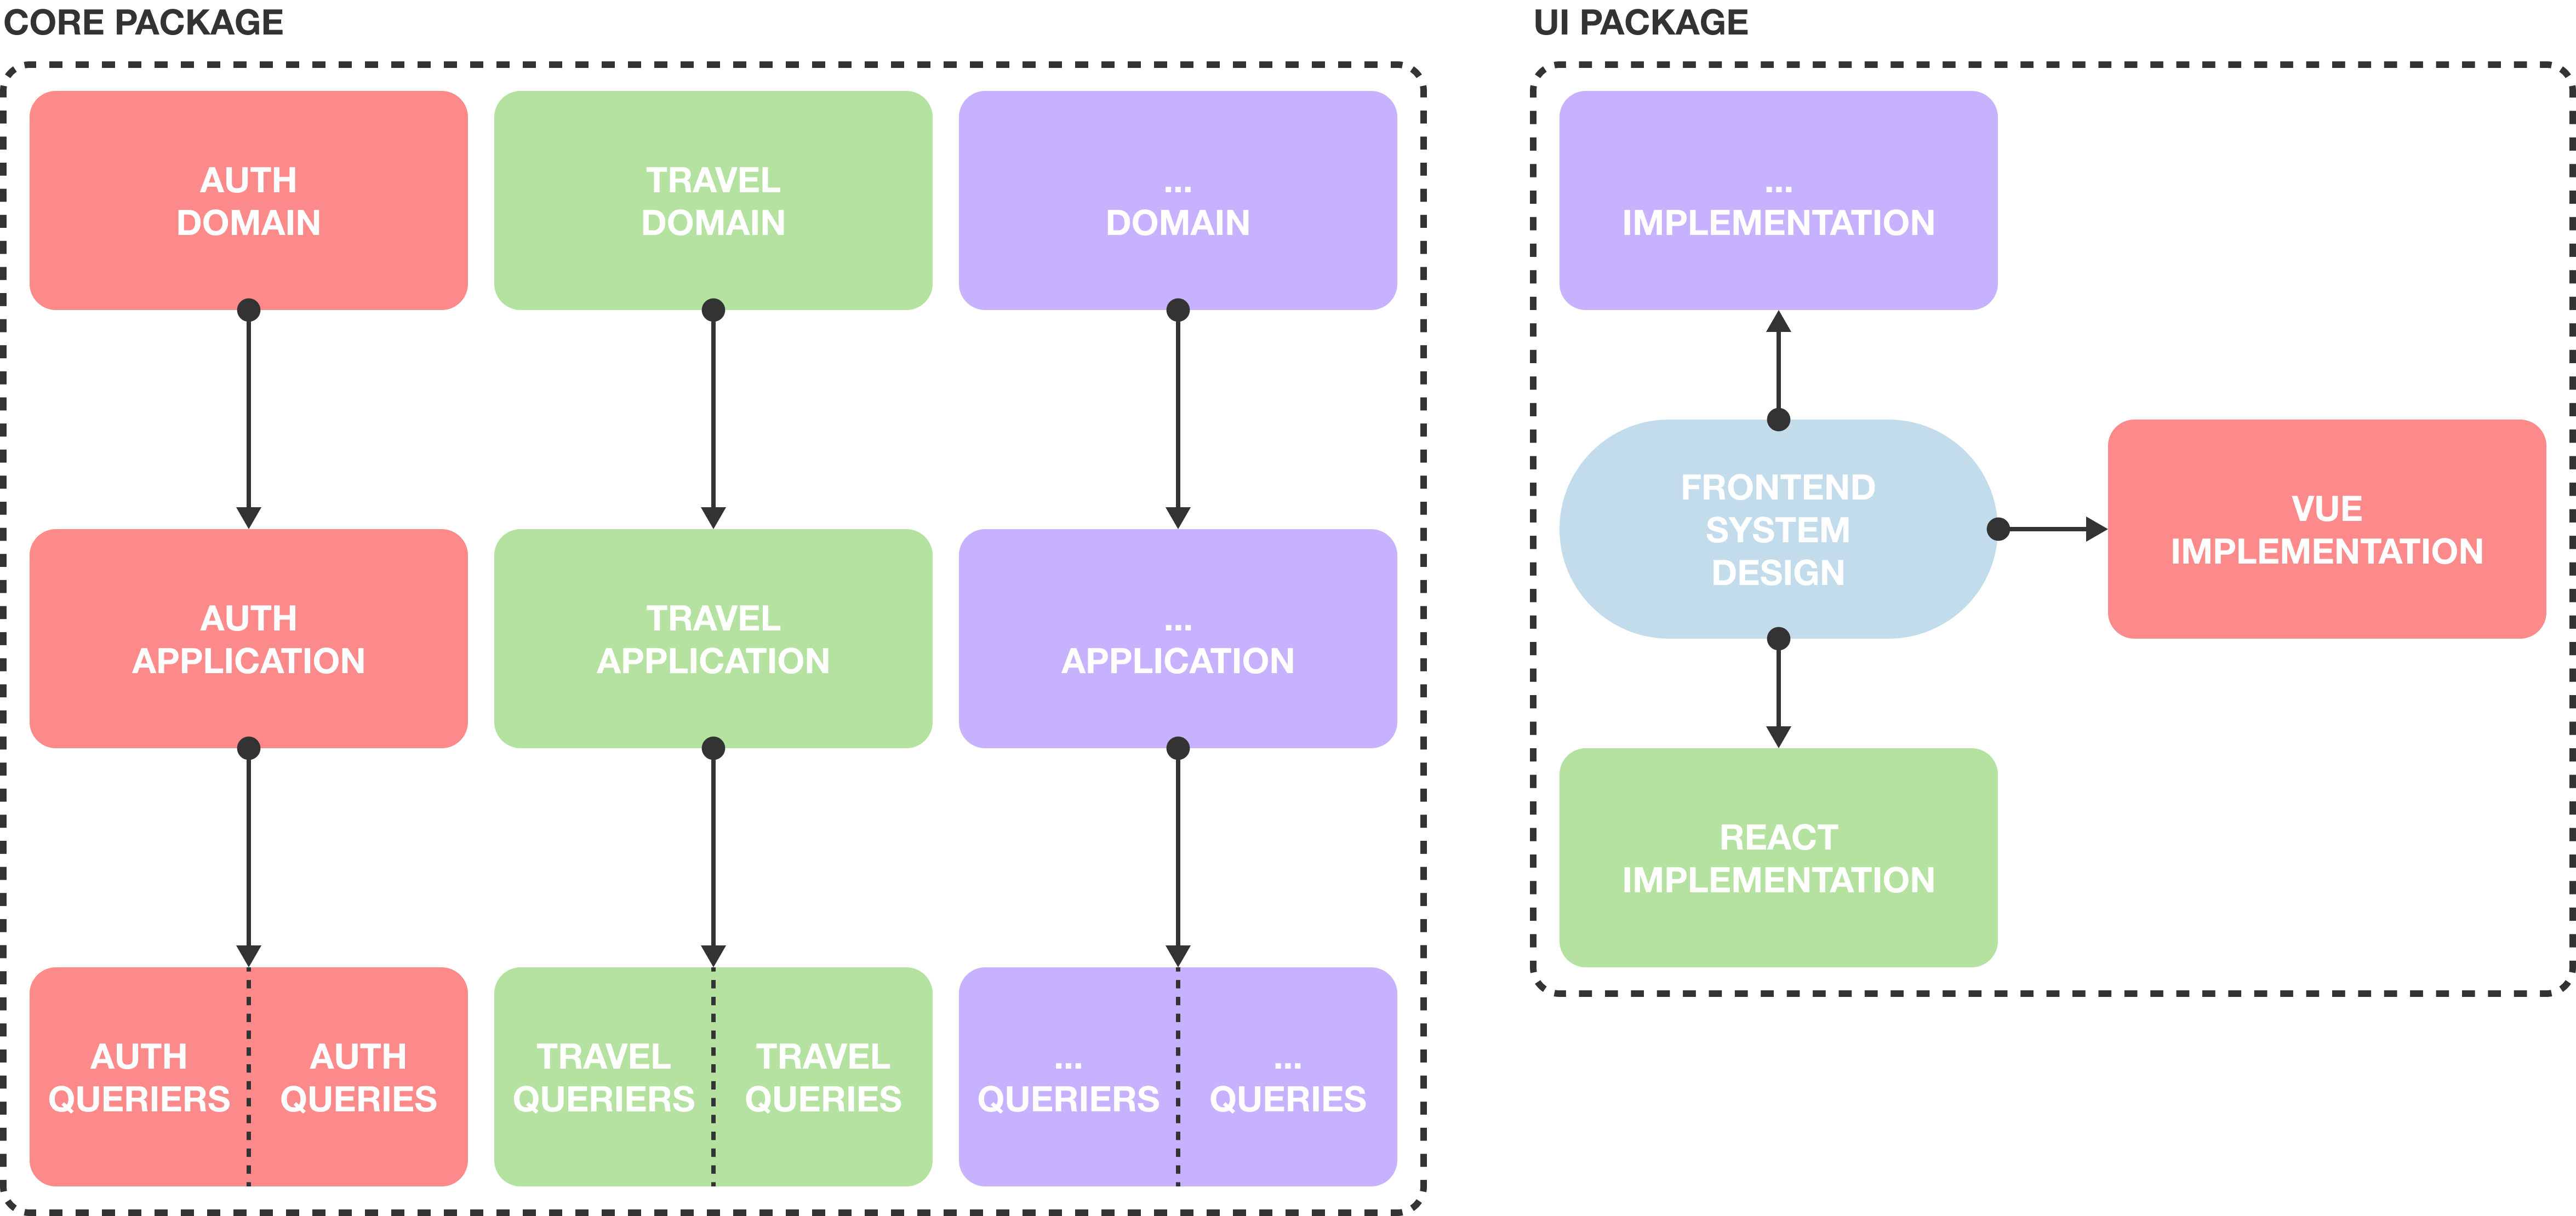
\includegraphics[width=\textwidth]{./assets/ui-core.png}
	\caption{Combination of core and UI packages.}
\end{figure}
It is important to mention that the \emph{System Design} pill should not be an
implementation, rather a specification, defined and maintained by the UI/UX
team. Since there was not enough time to develop a system design, this box does
not exist in the project current status.
\subsection{Site application}
Last but not least is the Nx application, which serves as the front-facing layer
of our architecture and contains the Next.js application that the users will
interact with. This layer is tightly coupled with the framework and leverages
the functionality provided by the core and UI layers to deliver a performant and
intuitive user experience.
\\[8pt]
While the Nx application itself is crucial, its source code becomes remarkably
streamlined and simplified. This is due to the fact that all the domain logic,
including API calls and validation, resides within the core package. Similarly,
the base implementation of components is contained within the UI package. With
this separation of concerns, the Next.js application can focus primarily on
state management and elements that enhance the user experience, such as
animations, performance optimizations, resource caching, and other related
aspects.
\\
By detaching the domain logic and component implementation to the core a UI
layers, the site application will contain a clearer and conciser codebase. This
separation improves code maintainability, since modifications in either
components or domain logic can be made in the respective layers, without having
a direct impact to the frontend. Furthermore, this separation also allows the
possibility of different releases per package, as explained in previous
chapters.
\\[8pt]
The implementation of the site package will be explained in the following
chapter, as it will focus on such implementation, explaining the decisions taken
in order to use all the power of Next.js, in order to provide a better user
experience. To sum up with this chapter, the integration of the site package
with the previous packages is:
\begin{figure}[H]
	\centering
	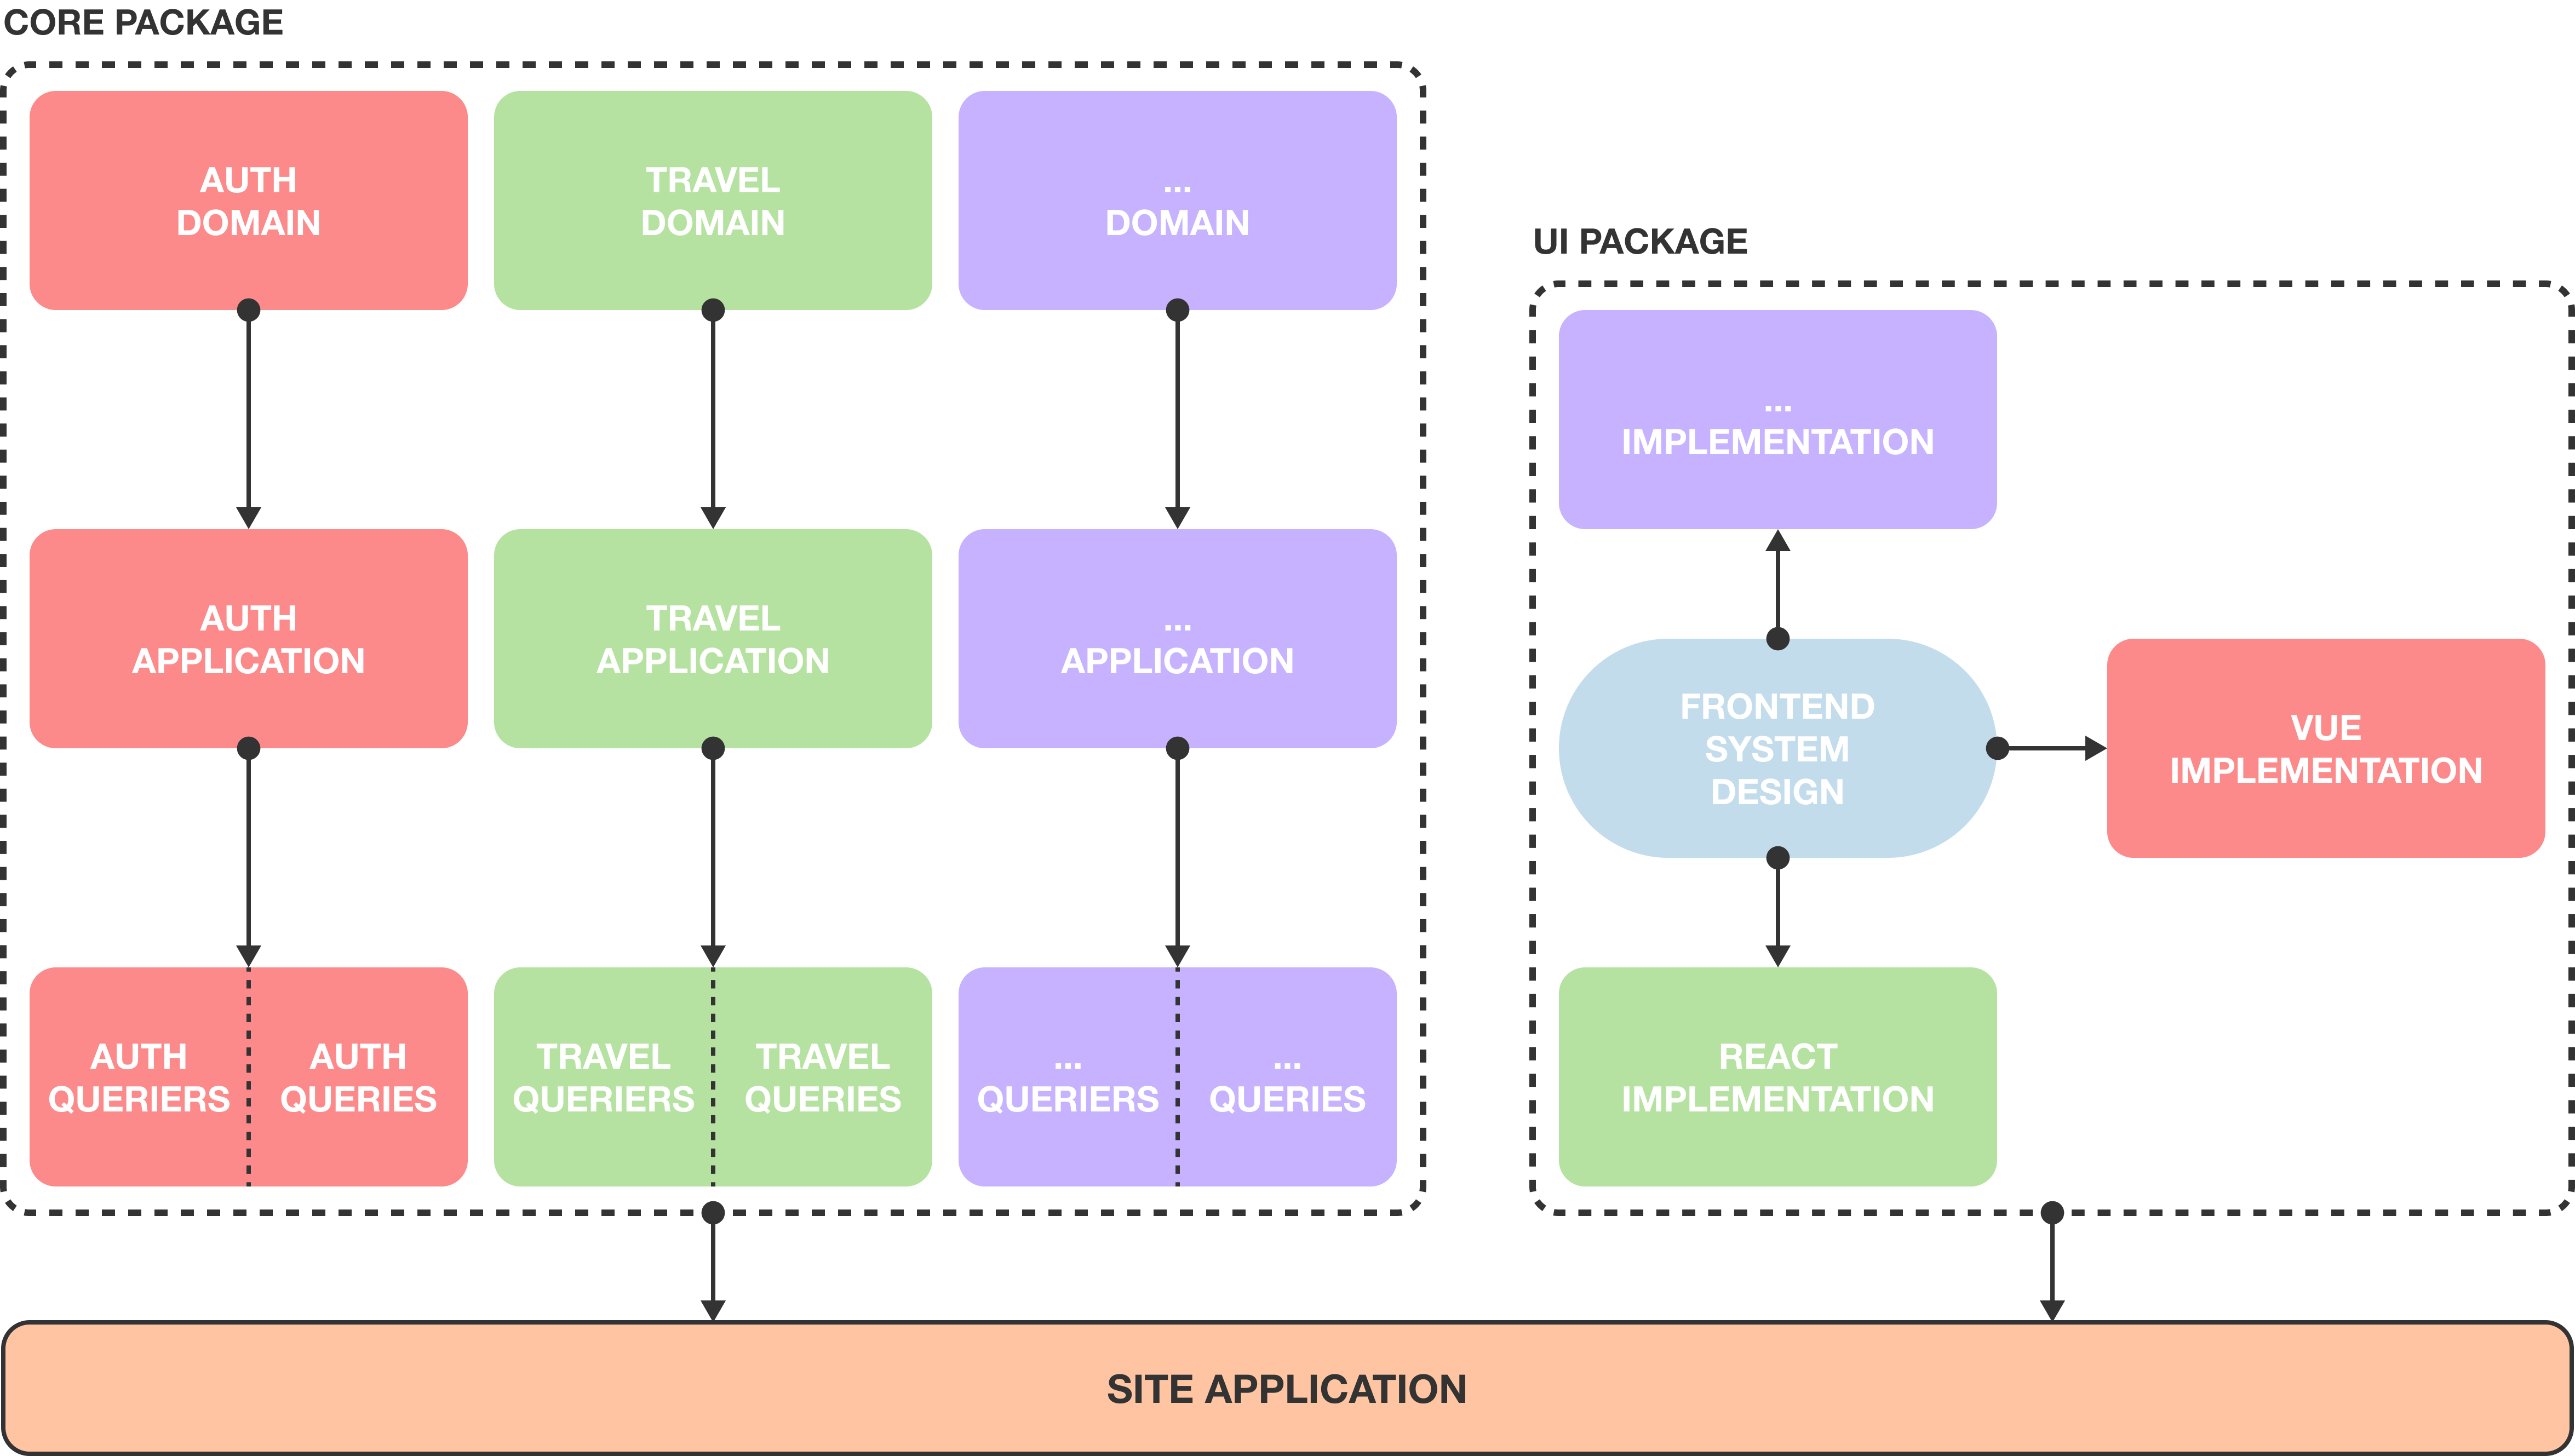
\includegraphics[width=\textwidth]{./assets/ui-core-site.png}
	\caption{Package structure including core, UI and site}
\end{figure}
\end{document}
